% !TEX root = ../main.tex

\section{introduction}
\label{sec:org662677c}





\subsection{Why is this important?}

Multilabel classification problems arise when multiple labels can be assigned during a prediction. Currently, research has produced no method to solve multilabel classification with an unknown number of labels. Rather, the literature reframes the problem as a multiclass problem, which effectively treats the classification as mutually exclusive. 

When we want to classify media into genres, text, sound, and images often belong to multiple genres. Hence, we need multilabel classification rather than multiclass classification. 

In this article, we are interested in higher-level concepts, for example genres, that can be mutually inclusive as opposed to mutually exhaustive. For example, a scientific journal can be tagged as \emph{machine learning} and \emph{economics}, a movie can be tagged as \emph{romance} and \emph{comedy}, a song might be considered \emph{jazz} and \emph{soul}. Among the candidate class labels, more than one of the candidate labels can be correct and the number of correct labels is unknown a priori. 

\mvm{In the multiclass paradigm, romance and comedy can be "romantic comedy". Why is that worse than having multiple labels? That's what the introductory literature review next should explain} 

\mvm{What is a higher-level concept?}

There is no reason why the earlier mentioned movie also cannot be an action movie–surely, the era-defining movie Spy is story of love, comedy, \textit{and} action. This article, thus, presents a framework for a problem formulation  SIMPUL, that is \textbf{S}ingle-\textbf{I}nstance \textbf{M}ultilabel \textbf{P}rediction for \textbf{U}nknown \textbf{L}abel counts, and a method to solve this problem, \emph{sigmoidF1}. 

\subsection{Literature}


\begin{itemize}[leftmargin=*]


\item \mvm{Multiclass versus multilabel? }

There seems to exist a consensus over the terms \emph{multiclass} and \emph{multilabel learning}, meaning mutually exclusive and mutually inclusive labels \footnote{definition mutually inclusive: they can overlap }, respectively~\cite{multilabelMethods}. Multilabel learning can therefore be seen as a subdomain of multiclass learning, where more than one class can be correct for the same example. 

\item \mvm{How does the literature reframe the problem?}


multilabel --> multiclass 


\item \mvm{How do you address this in abstract terms? }

Within multilabel training, we introduce the distinction between multi-instance multilabel~\citep[e.g.,][]{multiInstance, multiInstanceMultiLabel} and uni-instance multilabel. The term instance refers to segments in say a text or image that can be isolated as predictive of one or more labels, typically objects in an image. We define uni-instance learning as the case where the whole image / text / sound is predictive of a label; or at least if, with the current methods, it is not possible to isolate segments\footnote{Segments can be understood loosely here: a segment could be a detected interaction between 5 different expressions in the text that are together predictive of a label.} as predictive of certain labels.
\daan{I like how we are getting to a clear definition here. I am not sure if the uni vs multi-instance is really of importance. It could also maybe just be one sentence: note that in this work we do not consider the case of multi-instance ...}
% Multi-instance multilabel classification refers to labelling segments of images or text where training labels are typically only available at the image or document level. 
% \mdr{vague: Multi-instance multilabel classification refers to tasks where elements within each example can be singled-out and assigned one or more labels; examples include objects in an image or tokens in a text.}
% Uni-stance multilabel classification is \mdr{define it}.
% \mvm{the distinction between uni-istance and multi-instance also really confuses me and I don't see how it helps your argument}


\item \mvm{How does this fit in the literature}
\end{itemize}



\subsection{Proposition}


\begin{itemize}
\item technical problem definition
\begin{itemize}
	\item the number of labels is unknown a priori 
\end{itemize}


\end{itemize}

Mulitlabel classification problems with an unknown label count present numerous challenges. 

The first is that we do not know the number of labels is unknown a priori. 


\mvm{parapgraph below should only do one thing}


Machine learning prediction tasks' output are probabilistic (or a reversible transformation of a probabilistic measure such as a sigmoid or a soft max function). At training time, these probabilistic values are compared to binary values in the case of binary encoding of classes. At inference time, if the number $n_i$ of labels to be predicted per example is known a priori, it is logical to assign the $top_{n_i}$ predictions to that example~\cite{lossTopKError, topKmulticlassSVM}. If the number of labels per example is unknown a priori, the question remains at inference time as to how to extract information about the number of labels to assign to each example, beyond the propensity of labels to be assigned. This is generally done via a \emph{decision threshold}, that can be set globally for all examples. This threshold can optimize for specificity or sensitivity~\cite{decisionThreshold}.

\mvm{I don't see how these paragraphs flow into each other}

Little work can be found in the literature for \textbf{S}ingle-\textbf{I}nstance \textbf{M}ultilabel \textbf{P}rediction for \textbf{U}nknown \textbf{L}abel counts. We propose SIMPUL, a loss framework that accommodates for this gap in the literature. The existing measures to deal with SIMPUL can be divided into problem transformation (reverting back to a known problem formulation) and algorithm adaptation (adapting existing classification algorithms for the problem at hand). In the former case, cross-entropy losses are used at training time and thresholding is done at inference time. In the latter, elements of the learning algorithm are changed (such as the backpropagation procedure or the tasks). We propose a solution aligned with the algorithm adaptation paradigm, where we propose a custom loss formulation to solve SIMPUL problems.
\daan{I like that we can formulate this as a framework, but I wonder if we really need two new labels, SIMPUL and SigmoidF1. Maybe we should keep only one?}



 %We propose a loss framework based on confusion matrix metrics as losses. They have in common that they require step functions that are not decomposable for SGD. Hence, we propose a soft thresholding method with a sigmoid function to remedy this. \mvm{I would remove this altogether}



This is particularly fitting to the new models which are able to learn abstract labels from abstract representations.
Some of these metrics-as-losses can be particularly useful for tackling problems


Neural network models are able to learn increasingly more abstract representations via deeper networks, representation learning and self-supervision~\citep[see, e.g.,][]{SS,Rep}. Hence, we would expect that they also get better at predicting more abstract labels. 

Beyond identifying object types (see \cite{YOLO} and its successors), performing face recognition (see \cite{FaceNet} and its successors) on segments of an image, neural networks should soon be able to predict genres/categories of text, image and sound at high levels of accuracy. 

Towards this goal, there is a significant volume of recent work on building neural networks with a high-level of abstract understanding in the embedding space~\mdr{REF}.

However, there seems\daan{vague} to be limited research on developing loss functions that are adapted for these higher level concepts in the output space.

% \mdr{Briefly and concretely describe the abstract labeling task that we are interested in.}

% paper that uses mutually inclusive https://paperswithcode.com/paper/smile-semantically-guided-multi-attribute/review/
% https://www.diva-portal.org/smash/get/diva2:1324807/FULLTEXT01.pdf




% Coming back to the example of a scientific paper and its tags, it seems now clear that it is a multiclass multilabel learning problem, since several tags can be attributed to the same paper at once from different tag candidates. It is also arguable that it is a single-instance problem because it would be arguably hard to isolate expressions or interactions of expressions in a text that are predictive of a label. The prediction of mutually inclusive scientific paper categories is the main task to of this research.

% \mvm{I don't really see how the above paragraph is relevant, except } 





\begin{figure}[htbp]
\centering
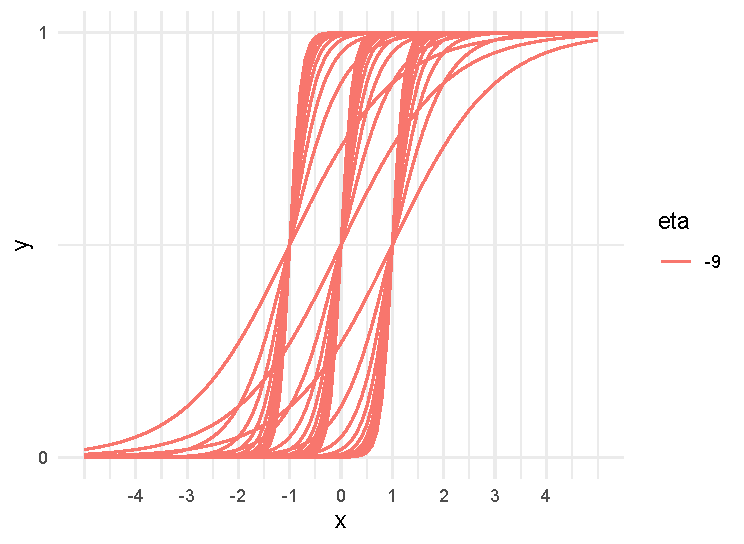
\includegraphics[width=.9\linewidth]{./images/sigmoid.pdf}
\caption{\label{fig:sigmoid}
Sigmoid function with different values for $\beta$ (steepness) \& $\eta$ (offset)}
\end{figure}

% \begin{itemize}
% \item \mdr{Now explain that the task introduced in the second paragraph is an instance of uni-instance multilabel classification.}
% \item \mdr{Now make the distinction between fixed label counts and varying label counts}
% \item \mdr{Little work has been done on the uni-instance, ML MC prediction with a varying number of classes}
% \item \mdr{Identify the shortcomings o prior work on the task that we care about}
% \end{itemize}

\begin{figure}[t]
\centering
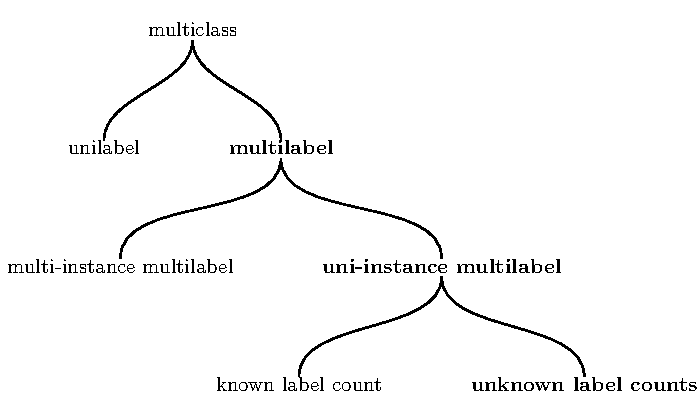
\includegraphics[width=.9\linewidth]{./tree/Tree.pdf}
\caption{\label{fig:tree}
SIMPUL (bold) within the \emph{multiclass} nomenclature
% Clarifying ``multiclass'' classification problems.
% In this paper we focus on the uni-instance, multilabel, multiclass classification problem with a varying number of labels (the bottom right hand side of the tree).
}
\end{figure}
% \mdr{Image source ...}

Learning to Rank (the practice of using Machine Learning to sort documents according to their relevance) lead to the widespread use of certain metrics~\cite{LTR}. In a number of retrieval tasks, a model's out of sample accuracy is measured on metrics such as AUROC, F1 score, etc. These reflect an objective catered towards evaluating the model over an entire ranking. Due to the lack of differentiability, these metrics cannot be directly used as loss functions at training time (in-sample). A seminal study~\cite{optimizableLosses} derived a general framework for deriving decomposable surrogates to some of these metrics. We propose our own decomposable F1 surrogate tailored for the problem at hand.

We first propose a general mathematical formulation of uni-instance multilabel learning for varying amounts of groundtruth labels. The generalization encompasses different levels of complexity, from the classical cross-entropy loss up to the proposed loss function. \emph{sigmoidF1} is a F1 score surrogate which allows to optimize for label prediction and count simultaneously in a single task and is robust to outliers.  \emph{sigmoidF1} and its adaptive \emph{SadF1} and Bayesian \emph{SBayesF1} counterparts are benchmarked against loss functions commonly used in multiclass learning and other existing models that are closely related to the SIMPUL setting. We show that our custom losses improve predictions over the current  state-of-the-art on several different metrics, across text and image related tasks.

The proposed contribution places SIMPUL tasks within the multiclass nomenclature. This shows a need for a specific mathematical formulation of the problem and particular tools to solve it. Our loss framework is tested on the Arxiv dataset which, to the best of our knowledge, makes this publication the first one using the entire breadth of that dataset published last August.


% \mdr{Now we have a paragraph in which you clearly describe your proposed line of attack}

% \mdr{Now we have a paragraph that explains the results that we have obtained with our proposed approach}

% \mdr{Now we have a paragraph with our main contributions:}
% \begin{itemize}[leftmargin=*]
% \item \mdr{Contribution 1}
% \item \mdr{Contribution 2}
% \item \mdr{Contribution 3}
% \end{itemize}

% \mdr{The remainder of the paper is organized as follows. Expand.}

% \vspace*{3cm}
% \mdr{Move all of the content to other sections, e.g., to background section or to related work. Also, try to avoid the meandering narrative that touches on many points but sometimes forgets to make explicit what its main point is.}



% \mdr{Too talkative, too many diverse angles. Make sure that there is a clear point that you are making:}
% Although multilabel binary prediction (commonly referring to mutually inclusive labels) is a task thoroughly covered in existing literature, there does not seem to exist a framework that deals with different amounts of positive labels in the groundtruth. For example, a scientific journal can be tagged as \emph{machine learning} and \emph{economics}, or a movie can be tagged as \emph{romance} and \emph{comedy}. These instances might as well be assigned only one tag in the groundtruth, or many more within the possible tags (classes).


% The particularity of tasks like scientific paper tagging or movie genre classification is that it remains unclear what elements in an image/video or text can be singled out as predictive of a particular tag/genre. Rather, a complex interaction between these elements in the feature space steer the predictions. For example, the sole mention of the term "machine learning" in a paper should not be a sufficient condition to tag it as such. Instead, one could expect from the publisher to get acquainted with the paper enough to determine wether the research is a worthwhile contribution or application of \emph{machine learning} to deserve the tag. This involves thorough understanding of the proposed method and background knowledge on state-of-the-art methods. An analogous argument can be made for movie genre classification for movie posters.

% However, if elements in an image/text can be singled out as predictive of a single tag, the problem reverts back to predicting with the a priori knowledge of the existence of only one true label (i.e. multi-instance multilabel learning).  The reason for distanciating singling-out from uni-instance labels, is that it has been shown that as soon as singling-out is possible, models that work on instances are more accurate \todo{rewrite this paragraph and sources}. 



% Common loss functions such as cross-entropy loss (for mutually inclusive labels) or multinomial logit loss (for mutually exclusive labels) deliver predictions on the unit interval. Thresholding the output to assess the performance of the model against the groundtruth can be done after training for (I), (II), (III) and (IV). \todo{give a very sound reason as to why we'd rather not do things post-training and rather at training-time}. Problem formulations (V), (VI) and (VII) suggest a solution at training time. We think that a custom loss function (VII) is the best alternative. \todo{explain why}



%%% Local Variables:
%%% mode: latex
%%% TeX-master: "../main"
%%% End:
